%% ----------------------------------
%%   Kap0---Grundlagen.tex
%% ----------------------------------

%% Grundlagen zum Verständnis und
%% Vergleich mit existierenden Arbeiten: Wieso können die die Zielsetzung nicht erfüllen?

\chapter{Grundlagen}
\label{sec:Chapter2}
In diesem Kapitel wird zu Beginn ein kurzer Überblick über Memristoren vermittelt. Danach sollen wissenschaftliche Arbeiten betrachtet werden, welche ähnliche Ansätze wie diese Bachelorarbeit verfolgen oder eine wichtige Rolle in dieser Bachelorarbeit spielen werden. Aufgeteilt ist die Betrachtung der anderen wissenschaftlichen Arbeiten in die drei Teilgebiete, auf welche im Zuge dieser Bachelorarbeit speziell Bezug genommen werden soll: Die Qualität, die Lebensdauer und die Formbarkeit von Memristoren. Die \glqq Qualität\grqq\,eines Memristors soll hierbei in der Bachelorarbeit mit einer Art von Note bewertet werden, welche von verschiedenen Faktoren beeinflusst wird. Auf diese Thematik wird im Kapitel 3 \glqq Konzept\grqq\,näher eingegangen. Außerdem soll die \glqq Lebensdauer\grqq\,eines einzelnen Memristors durch Berechnungen und Messungen approximiert werden. Zuletzt soll noch die sogenannte \glqq Formbarkeit\grqq\,eines Memristors untersucht werden. Hierbei soll dieser so beeinflusst werden, dass die Hysterese des Memristors eine gewünschte Form annimmt. In dieser Arbeit soll die Formbarkeit im Spezifischen überprüfen, wie formbar die Hysterese des betrachteten Memristors allgemein ist.

\begin{figure}
  \centering
    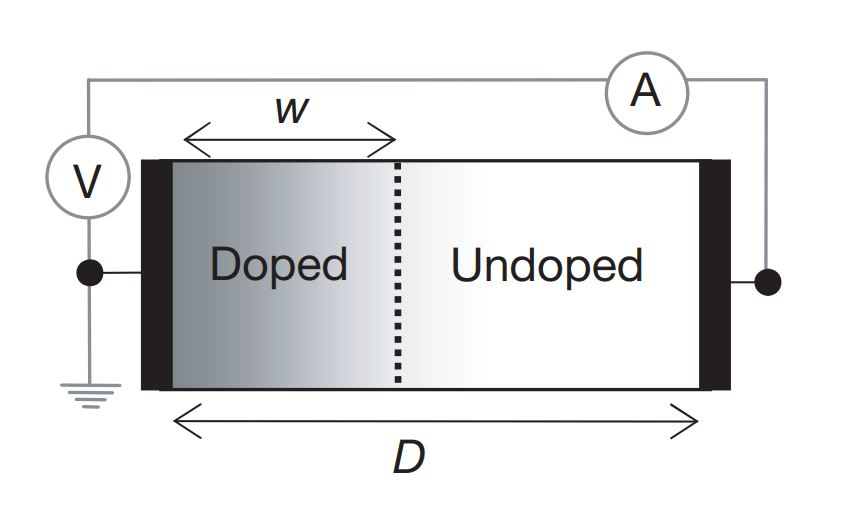
\includegraphics[width=0.5\textwidth]{images/hp_mem.JPG}
    \quelle{\cite{hp_2008}}
  \caption{HP Memristor Modell.}
  \label{fig:hp_mem}
\end{figure}

Bei dem Memristor, welchen Strukov et al.~\cite{hp_2008} 2008 entwickelten, handelt es sich um ein Schaltelement, welches aus zwei Platinelektroden besteht, die eine nicht dotierte Titandioxid (TiO$_2$) und eine dotierte Titandioxid (TiO$_{2-x}$) Schicht zwischen sich eingeschlossen haben, siehe Abb.~\ref{fig:hp_mem}. Die beiden unterschiedlich dotierten Titandioxid-Schichten entscheiden anhand ihrer Verteilung untereinander, wie leitfähig der Memristor ist. Der dotierte Titandioxid-Anteil hat einen sehr niedrigen Widerstand, welcher von Strukov et. al. mit $R_{\text{ON}}$ bezeichnet wird. Der Anteil des nicht dotierten Titandioxids hat einen sehr hohen Widerstand und wird dementsprechend $R_{\text{OFF}}$ genannt. Wird eine Spannung in eine der beiden Richtungen angelegt so verändert sich das Verhältnis zwischen den beiden dünnen Filmen aus Titandioxid. So wie sich der Anteil der dünnen Filmschichten in dem Memristor verändert, verändert sich dadurch die Leitfähigkeit beziehungsweise der Gesamtwiderstand des Bausteins.

Memristoren haben die Eigenschaft nicht flüchtig zu sein oder wie die Autoren der Arbeit~\cite{vde_memristor} schreiben:
\begin{quote}
  \textit{The device remembers its history}, [...]
\end{quote}
Falls keine Spannung am Memristor anliegt, so bleibt er in dem Zustand, welchen er abhängig von der zuletzt angelegten Spannung erreicht hat. Er merkt sich sozusagen, welcher Strom in der Vergangenheit angelegt war. Solange kein Strom auf den Memristor angelegt wird, bleibt er starr auf dem aktuellen Widerstand, was ihm seine memristive, also speichernde Eigenschaft verleiht.



Das Memristor-Modell, welches von HP entwickelt wurde, wird von den meisten wissenschaftlichen Arbeiten betrachtet und verwendet. Doch HP ist nicht das einzige Unternehmen, welches Memristoren erforscht und produziert. Es gibt viele Modelle von anderen Wissenschaftlern und Unternehmen~\cite{team_model,elec_model,spice_model}, welche an einer anderen Möglichkeit arbeiten, um den von L.Chua vorgestellten Memristor~\cite{chua_mem} in die Realität umzusetzen. So gibt es zum Beispiel PCM (Phase Change Memory), ReRAM (Resistive RAM), MRAM (Magnetoresistive RAM), STT-RAM(Spin-Transfer Torque RAM) und NRAM (Nano RAM), welche alle verschiedene Realisierungen von memristiven Systemen sind. Nähere Information zu den verschiedenen Arten von Memristoren werden in der Arbeit~\cite{vde_memristor} beschrieben. Knowm Inc. gehört zu den genannten Unternehmen, welche an alternativen Realisierungen des Memristors arbeiten und diese leicht verfügbar machen wollen. Aus diesem Grund wird in dieser Arbeit die von Knowm vorgegebene Umgebung zur Forschung von Memristoren genutzt.

\begin{figure}
  \centering
    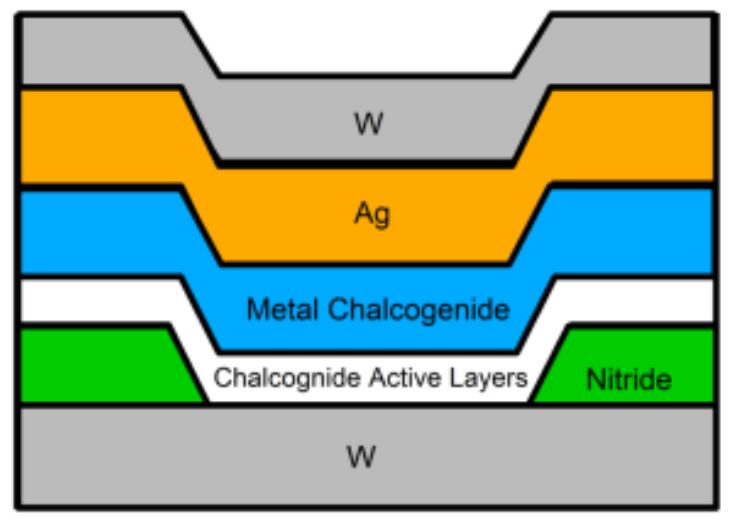
\includegraphics[width=0.65\textwidth]{images/Knowm_Mem.jpg}
    \quelle{\cite{knowm_comp_2015}}
  \caption{Knowm Memristor Material Modell.}
  \label{fig:knowm_mem}
\end{figure}

Der Knowm-Memristor unterscheidet sich in einigen Punkten von dem 2008 erstellten Memristor von HP, besitzt aber im Grunde die gleichen Eigenschaften eines Memristors. Wie in Abb.~\ref{fig:knowm_mem} bereits zu erkennen ist, setzen Alex Nugent und das Team von Knowm nicht auf Platinelektroden und Titandioxid für ihren Memristor. Für die Elektroden gibt es drei mögliche Varianten, welche Knowm zum Verkauf zur Verfügung stellt: Wolfram (W), Zinn (Sn) und Chrom (Cr). Alle Varianten schließen ein leicht oxidierbares chalkogenides Metall ein, welches durch Anlegen von Strom eine aktive Schicht nahe der Elektrode mit dem niedrigeren Potenzial bildet. Diese Schicht hat eine höhere Leitfähigkeit, was wiederum gleichzusetzen ist mit einem niedrigeren Widerstand. Durch die Bipolarität des Geräts lassen sich hohe und niedrige Widerstände erreichen, was dem Gerät einen memristiven Charakter gibt und ihn damit als Memristor klassifiziert.
Knowm hat sich gemeinsam mit der Materialforscherin Kris Campbell für diese Architektur entschieden, da sie ihre Memristoren mit der Absicht herstellen wollten, diese der Öffentlichkeit zugänglich zu machen. Nach ihrer Meinung ist der Titandioxid Memristor von HP zu kompliziert und fehleranfällig in der Herstellung. Auch ist der von Knowm produzierte Memristor nach eigenen Angaben weniger anfällig auf äußere Einflüsse, was ihn massentauglicher machen soll.


\section{Vergleichbare existierende Ansätze in Hinblick auf die Qualität}
\label{sec:Qualität}
Wissenschaftliche Arbeiten, welche sich auf die Qualitätsunterschiede von einzelnen Memristoren beziehen, gibt es nach aktuellem Stand nicht. Knowm beschreibt in ihrer Arbeit zu ihrem Memristor jedoch einige Messdaten zu ihren Memristoren, welche genutzt werden können, um ein Qualitätsmaß anzusetzen~\cite{knowm_comp_2019}. Memristor Discovery ist die zum gleichnamigen Knowm Memristor Discovery Board V2 gehörende Sofware aus dem Hause Knowm, mit welcher einige Messungen und Tests an den Memristoren durchgeführt werden können. Ein Screenshot der Software ist in Abbildung~\ref{fig:knowm_discovery}~ zu sehen. Diese Software ist Open Source und bietet damit eine Grundlage für diese Bachelorarbeit. Es ist möglich mit der Software die Hysteresen der Knowm eigenen Memristoren zu messen und händisch durch Regler zu verändern. Mit dem sogenannten \glqq Boardcheck\grqq\,gibt es eine Funktion, die erkennen lässt, ob ein Memristor noch lauffähig ist oder nicht. Jedoch wird bei diesem Boardcheck nur getestet, ob überhaupt der Memristor in einen zulässigen Widerstandsbereich liegt. Ein zulässiger Widerstand ist bei diesem Check ein Widerstandswert, welcher im von Knowm festgelegten Bereich von Widerständen der Memristoren liegt. Die Grenzwerte dazu finden sich in dem Knowm Datenblatt~\cite{knowm_comp_2019}. Jedoch wird keine Aussage über die Qualität eines einzelnen Memristors getätigt.

\begin{figure}
  \centering
    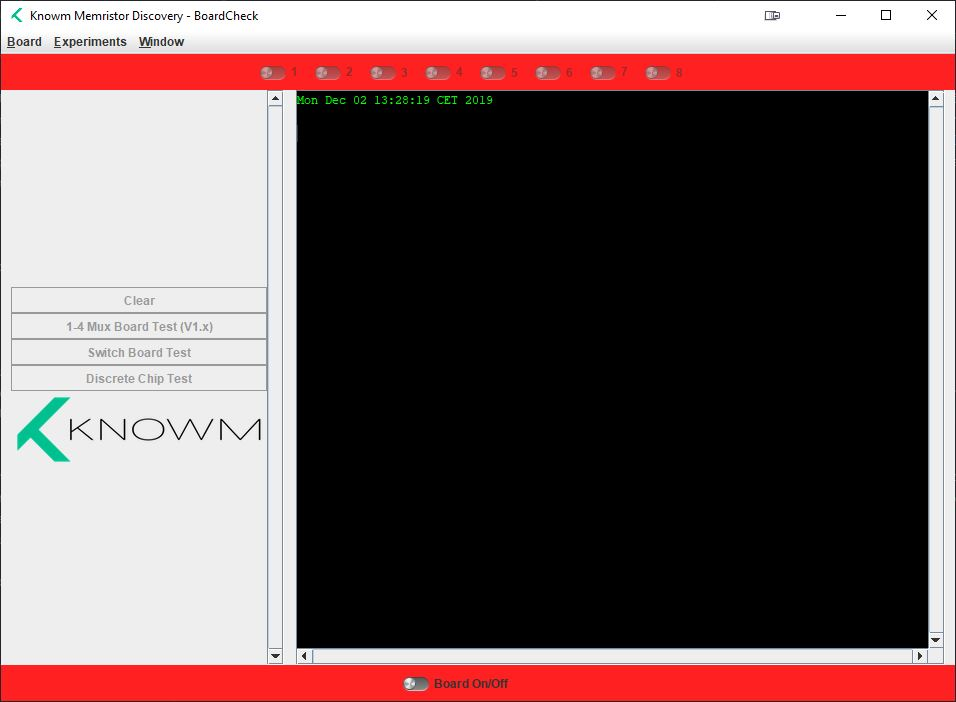
\includegraphics[width=0.8\textwidth]{images/Memristor_Discovery_tmp.jpg}
  \caption{Knowm Memristor Discovery Software \glqq Board Check\grqq.}
  \label{fig:knowm_discovery}
\end{figure}

Mit der allgemeinen Qualität von Memristoren befasst sich die Arbeit von Perez und De Rose~\cite{nonvolatile}. Die Autoren vergleichen hierbei herkömmliche Speichermedien mit dem RRAM. Die aus der genannten Arbeit übernommene Tabelle in Abbildung~\ref{tab:DRAM/RRAM} vergleicht die beiden Arten von Speichermedien anhand einiger Metriken. Ein sehr auffälliges Merkmal, bei dem sich DRAM und RRAM unterscheiden, ist die Kapazität. RRAM kann laut den Autoren die zehnfache Menge von DRAM an Gigabytes auf einem Quadratzentimeter speichern. Ein anderes sehr auffälliges Merkmal ist die Lebensdauer, auf welche in dieser Arbeit noch näher eingegangen wird. DRAM besitzt eine Haltbarkeit von ungefähr $10^{10}$ Schreibzyklen, RRAM dagegen mit $10^5$ Schreibzyklen viel weniger. Jedoch wird die Qualität von Memristoren in dieser Arbeit sehr allgemein gehalten und bezieht sich ausschließlich auf den Vergleich mit herkömmlichen Speichermedien und nicht untereinander.

\begin{figure}
  \centering
  \begin{tabular}{|c|c|c|c|}
    \hline\textbf{Metric} & \textbf{DRAM} & \textbf{RRAM} & \textbf{Advantage} \\\hline
    Capacity (GB/cm$^2$) & 46 & 466 & RRAM \\\hline
    Area Efficiency & Less & More & RRAM \\\hline
    Write Speed (ns) & 10, round trip & 10, just one cell & DRAM \\\hline
    Read Speed (ns) & 10, round trip & Uncertain, likely better & RRAM \\\hline
    Yield & 90\% & 80-95\% & tie \\\hline
    Retention Time & 16ms & 2yr & RRAM \\\hline
    Readability & 10$^{-1}$ & 10$^5$ & RRAM \\\hline
    Endurance & 10$^{10}$ write cycles & 10$^5$ write cycles & DRAM \\\hline
  \end{tabular}
  \quelle{\cite{nonvolatile}}
  \caption{Vergleich von DRAM und RRAM anhand einiger Metriken.}
  \label{tab:DRAM/RRAM}
\end{figure}

In der wissenschaftlichen Arbeit~\cite{char_mem} vergleichen die Autoren das HP Memristor Modell mit anderen existierenden Modellen, darunter auch das von Knowm Inc. Hierbei werden beispielsweise die I-V Charakteristiken und daraus resultierenden Hysteresen analysiert und unterschieden. Jedoch betrachtet auch diese Arbeit nicht die Qualität von einzelnen Memristoren. Es wird vielmehr ein Schwerpunkt auf den Vergleich von allgemeinen Modellen gelegt und dabei untersucht, wie diese sich verhalten. So werden in der Arbeit, wie an Abbildung~\ref{fig:char_mem} zu erkennen ist, beispielsweise Daten zu verschiedenen Memristor Modellen gesammelt und die I-V Charakteristiken und die Hysteresen in graphischen Darstellung verglichen und analysiert.

\begin{figure}
  \centering
    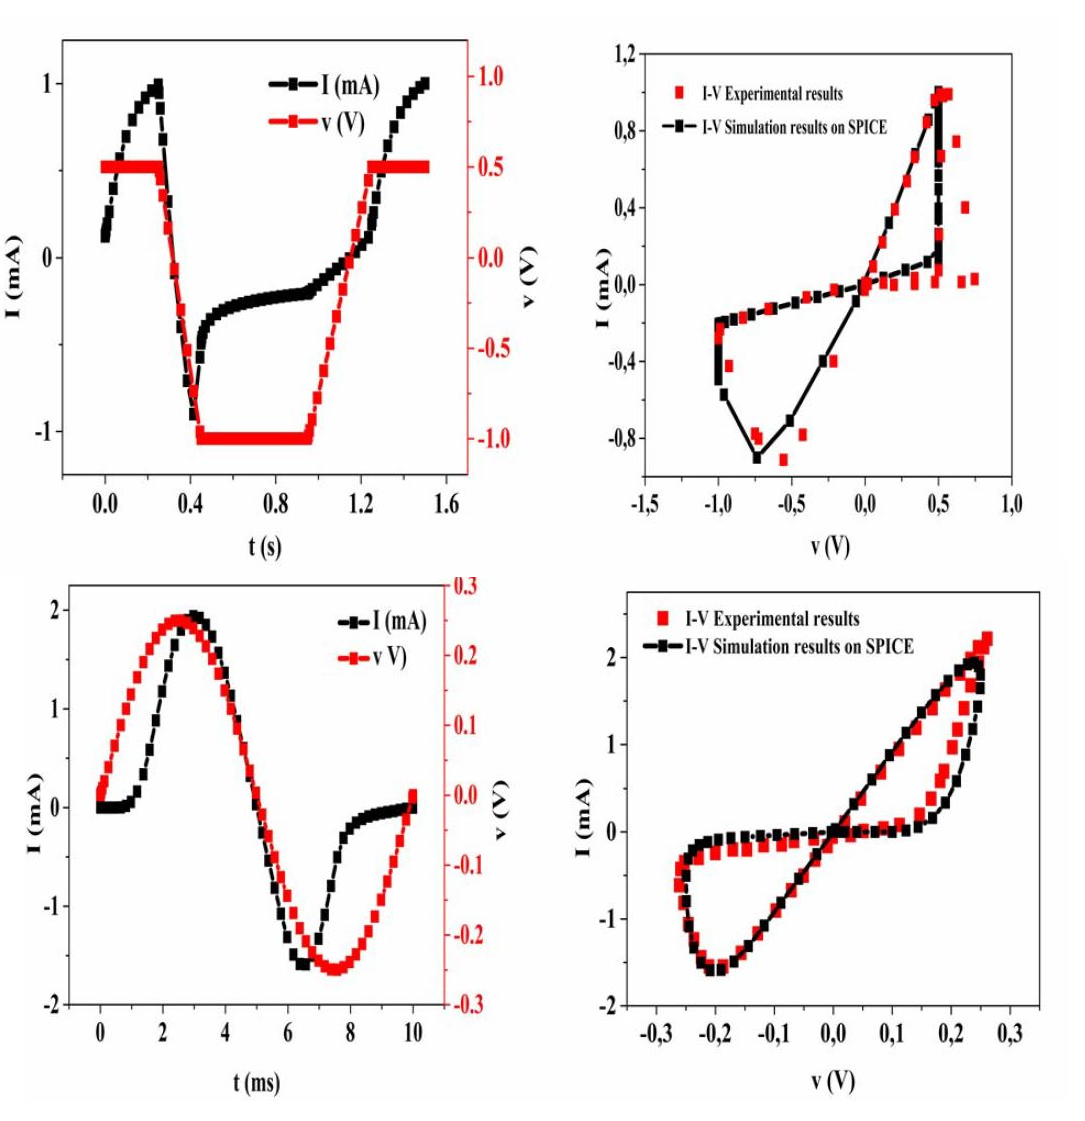
\includegraphics[width=0.6\textwidth]{images/Charcterization_Mbarek.png}
    \quelle{\cite{char_mem}}
  \caption{Vergleich von verschiedenen Modellen, hier zwischen Strachan (oben) und Nugent/Knowm (unten).}
  \label{fig:char_mem}
\end{figure}

\section{Vergleichbare existierende Ansätze in Hinblick auf die Lebensdauer}
\label{sec:Lebensdauer}
Die Arbeit~\cite{stat_lifetime} begutachtet die sogenannten \glqq memristive Crossbar-Architekturen\grqq\, und analysiert die Lebensdauer dieser Systeme. Es wird untersucht, welche Gründe es dafür gibt, dass memristive Geräte mit der Zeit ihre Fähigkeit verlieren in einer Crossbar-Architektur zu funktionieren und ausgetauscht werden müssen. Laut der Autoren des Papers ist einer der Hauptindikatoren der Mechanismus von memristiven Systemen, bei dem der \glqq High Resistive State\grqq\,(HRS) mit der Zeit an Widerstand verliert und der Widerstand des sogenannten \glqq Low Resistive State\grqq\,(LRS) mit der Zeit zunimmt. Abbildung~\ref{fig:lebensdauer} zeigt hierbei die Abnahme des HRS und die Zunahme des LRS bis zu dem Zeitpunkt $\tau$ mit einer Widerstands-Differenz $\mathcal{K}$, an welchem der Memristor als nicht mehr funktionsfähig gewertet werden kann. Die Autoren beziehen sich in ihren Ausführungen auf die Arbeit~\cite{endurance_deg}, welche diese Mechanismen näher beschreibt. Außerdem stellen die Autoren in ihrer Arbeit fest, dass zur Berechnung der Lebensdauer einer Crossbar-Architektur von Memristoren erst einmal die Lebensdauer eines einzelnen Memristors bestimmt werden muss. Diese Erkenntnis und die darauf folgenden Berechnungen sind besonders interessant für diese Arbeit. Die Lebensdauer $\tau$ wird nach den Berechnungen und Analysen der Autoren wie folgt berechnet:
\begin{align*}
  \tau = \alpha \times HRS(0) - \beta \times LRS(0)
\end{align*}
Hierbei stellen $\alpha$ und $\beta$ Koeffizienten dar, welche von einem festgelegten $K$ für die minimale Differenz zwischen HRS/LRS und dem Abfall beziehungsweise der Steigung von HRS ($slope_{HRS}$) und LRS ($slope_{LRS}$) abhängt. $HRS(0)$ und $LRS(0)$ sind HRS und LRS zu dem Zeitpunkt, an welchem noch 0 Schreibzyklen durchlaufen wurden.

\begin{figure}
  \centering
    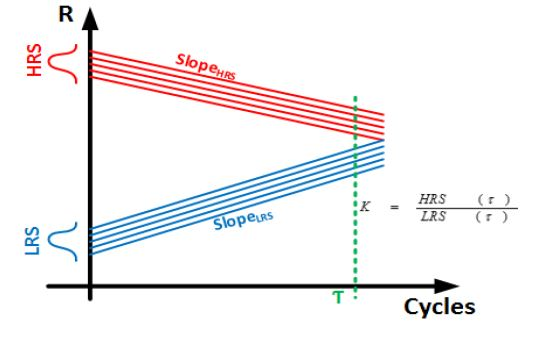
\includegraphics[width=0.7\textwidth]{images/Lebensdauer_Graph.jpg}
    \quelle{\cite{stat_lifetime}}
  \caption{Lebensdauer eines Memristors bis zum Zeitpunkt $\tau$. Der \glqq High Resistive State\grqq\,(HRS) und der \glqq Low Resistive State\grqq\,(LRS) nähern sich während der Lebenszeit eines Memristors an. Bei einem bestimmten Abstand zwischen HRS und LRS gilt der Memristor als nicht mehr funktionsfähig.}
  \label{fig:lebensdauer}
\end{figure}

\section{Vergleichbare existierende Ansätze in Hinblick auf die Formbarkeit}
\label{sec:Formbarkeit}

In Hinblick auf die Formbarkeit gibt es zum aktuellen Stand keine wissenschaftliche Veröffentlichung, welche sich auf einzelne Memristoren konzentriert. Das Paper~\cite{compact_model} bezieht sich nur im weitesten Sinne auf die Formbarkeit, indem es einen theoretischen, mathematischen Ansatz zum Formen einer Hysterese aufstellt. Hierbei kommt es weder zum Vergleich zwischen Memristoren, noch zum Aufstellen einer Charakteristik für einen einzelnen Memristor. Das Paper~\cite{exploring_mem} steht diesbezüglich dieser Arbeit um einiges näher. Die Autoren nutzen den von Knowm hergestellten Memristor und die dezugehörige Software. In dem Paper kommt es zu einer allgemeinen Charakterisierung des Knowm-Memristors. Für diesen Abschnitt ist jedoch wichtiger, dass die Hysterese eines Memristors untersucht wird. Hierbei werden verschiedene Spannungen angelegt und überprüft, wie sich die Hysterese verändert. Da es sich aber nur um einen kleinen Abschnitt im Paper handelt, welcher sich dabei sehr allgemein hält, hat auch dieser keinen großen Einfluss auf diese Bachelorarbeit.

\section{Die Relevanz dieser Arbeit}

Wie bereits in den vorherigen Abschnitten klar gemacht wurde, gibt es derzeit noch keine vergleichbare Arbeit auf dem Gebiet der Memristorforschung. Während die meisten wissenschaftlichen Arbeiten eher auf einer allgemeinen Ebene gehalten werden, soll diese Arbeit sich auf einzelne Memristoren beziehen. Memristoren unterscheiden sich aufgrund ihrer Herstellungsmethode oftmals stark voneinander, wie die Arbeit~\cite{auto_adjust} feststellt. Somit ist die Betrachtung von einzelnen Memristoren für bestimmte Anwendungsgebiete vorteilhaft. So kann es für bestimmte Anwendungsgebiete notwendig sein, dass ein Memristor möglichst viele verschiedene Zustände annimmt. Oder dass Memristoren, welche zusammenarbeiten, möglichst gleich viele Zustände annehmen können. Auch kann es sein, dass für bestimmte Anwendungsgebiete ein etwas höherer Schwellenwert, in folgenden Teil dieser Bachelorarbeit immer \glqq Threshold\grqq\,genannt, zu besseren Ergebnissen führt. Das Bestimmen der restlichen Lebensdauer eines Memristors spielt genau aus den gleichen Gründen eine sinnvolle Rolle. Wenn man erkennen kann, dass ein Memristor nicht mehr lange funktionieren wird, kann verhindert werden, dass solch ein Memristor in ein fest verlötetes System eingebaut wird. Eine Prognose über die zu erwartende Restlebensdauer eines Memristors ist für solche Fälle von großem Nutzen. Für bestimmte Forschungsanwendungen kann es außerdem von Vorteil sein, eine Hysterese eines Memristors in eine bestimmte Form zu bringen, da er somit bestimmte Charakteristiken annimmt, welche zum Beispiel einem anderen Memristor ähneln. Da die Memristor Discovery Software von Knowm diesen Ansprüchen nicht entgegen kommt, soll diese Arbeit derartige Optionen entwickeln.
